W wyniku testów wyłoniony został model o najlepszej dokładności realnej, tj.
dokładności klasyfikacji zewnętrznych grafów testowych.
Model ten okazał się jednym z najbardziej podstawowych z przygotowanych,
bo jest to podstawowy model uczony na grafach sześciowierzchołkowych.
W ramach eksperymentu, zastosowano dla niego modyfikacje,
które pomogły zwiększyć realną dokładność modelu.
Modyfikacje te zostały wprowadzone i przetestowane w podrozdziale z testami modeli
z walidacją krzyżową.
Jedyną zmianą z zaproponowanych, która przynosi realne korzyści,
jest zwiększenie liczby filtrów w warstwach sieci neuronowej, kolejno 32, 64 oraz 128 dla Conv2D,
oraz zastosowanie zwiększonego parametru dropout - 0,5.

\textbf{Zmodyfikowany model podstawowy uczony na grafach sześciowierzchołkowych}

Model osiąga poprawne wyniki, lecz po około 55 epoce procesu nauczania,
dokładność gwałtownie spada, aż do wartości około 23\%.

Ta sama sytuacja dotyczy straty, która to gwałtownie wzrasta około 60 epoki,
z około 0,25, do aż 1,75.

\begin{figure}[ht]
	\centering
	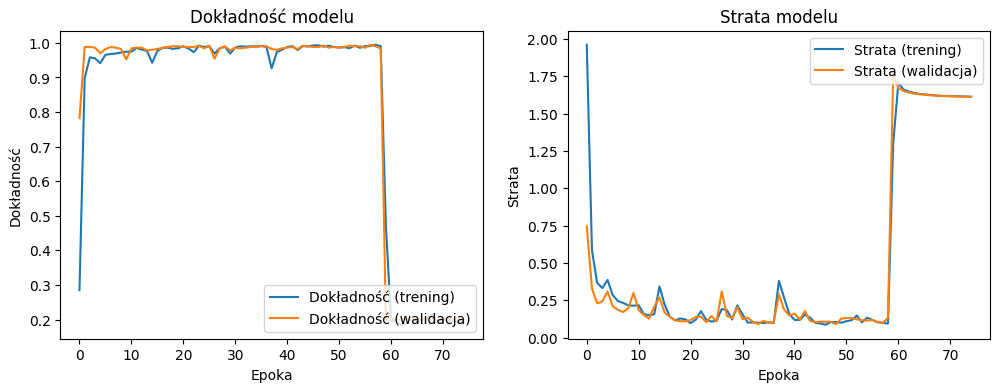
\includegraphics[height=5.5cm]{resources/tests/images/v4/base6_1_img.png}
	\caption{Wyniki testów dla zmodyfikowanego modelu podstawowego, liczba wierzchołków = 6}
	\label{Fig:tests-base-5a}
\end{figure}
\FloatBarrier

% \begin{figure}[ht]
% 	\centering
% 	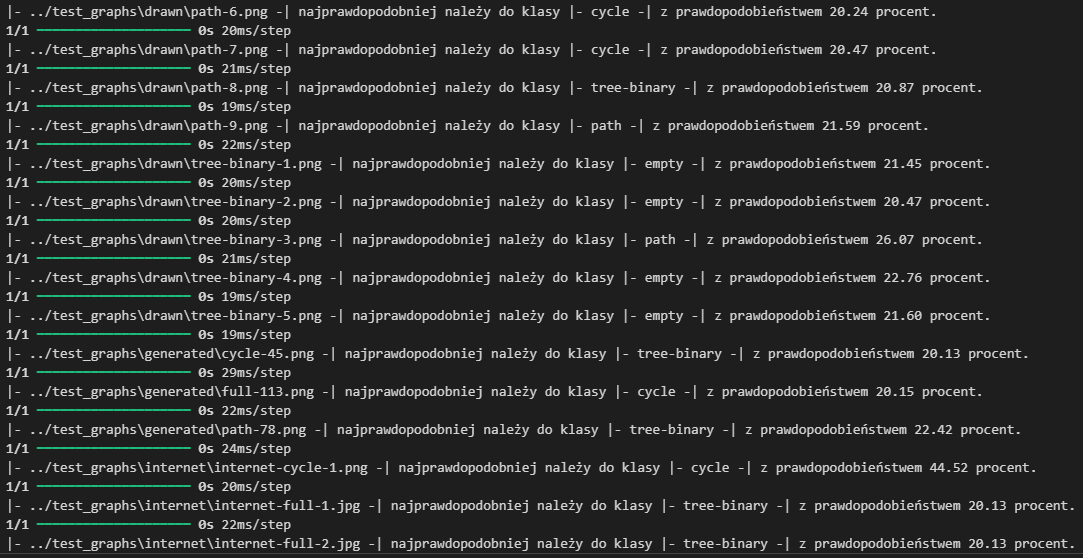
\includegraphics[width=14cm]{resources/tests/images/v4/base6_1_txt.png}
% 	\caption{Klasyfikacja obrazów zewnętrznych dla zmodyfikowanego modelu podstawowego, liczba wierzchołków = 6}
% 	\label{Fig:tests-base-5b}
% \end{figure}
% \FloatBarrier

% \begin{figure}[ht]
% 	\centering
% 	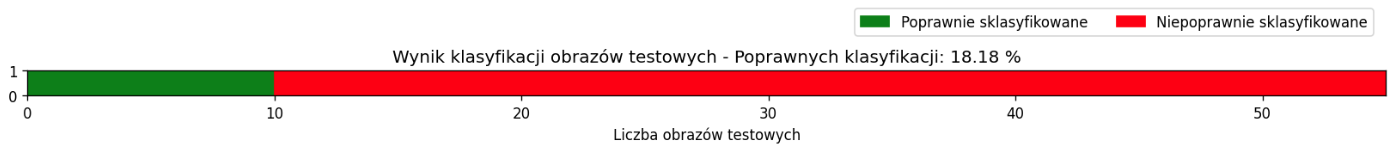
\includegraphics[width=14cm]{resources/tests/images/v4/base6_1_bar.png}
% 	\caption{Wizualizacja klasyfikacji obrazów zewnętrznych dla zmodyfikowanego modelu podstawowego, liczba wierzchołków = 6}
% 	\label{Fig:tests-base-5c}
% \end{figure}
% \FloatBarrier

\textbf{Zmodyfikowany poprawiony model podstawowy uczony na grafach sześciowierzchołkowych}

Wyniki uzyskane z procesu nauki poprzeniego modelu sugerują zmniejszenie liczby epok do około 55.
Taka modyfikacja została zastosowana, a test przeprowadzono ponownie.

% -- TO DO -- % Dokładność

% -- TO DO -- % Strata

\begin{figure}[ht]
	\centering
	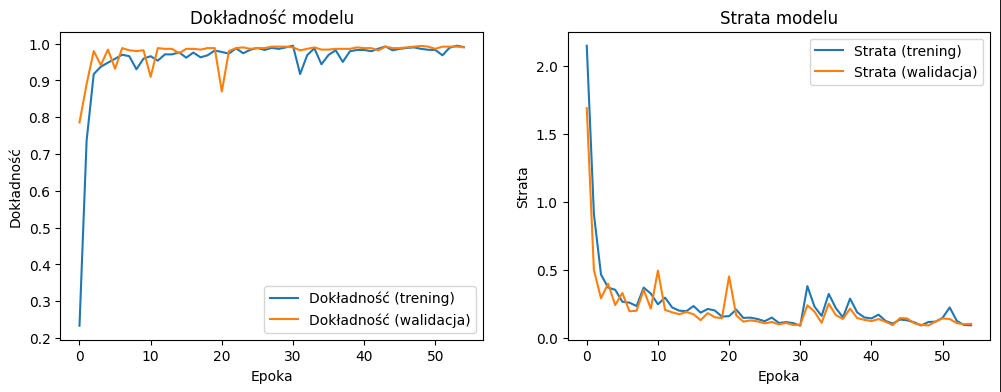
\includegraphics[height=5.5cm]{resources/tests/images/v4/base6_1_1_img.png}
	\caption{Wyniki testów dla poprawionego zmodyfikowanego modelu podstawowego, liczba wierzchołków = 6}
	\label{Fig:tests-base-6a}
\end{figure}
\FloatBarrier

% -- TO DO -- % Opis ogólny

\begin{figure}[ht]
	\centering
	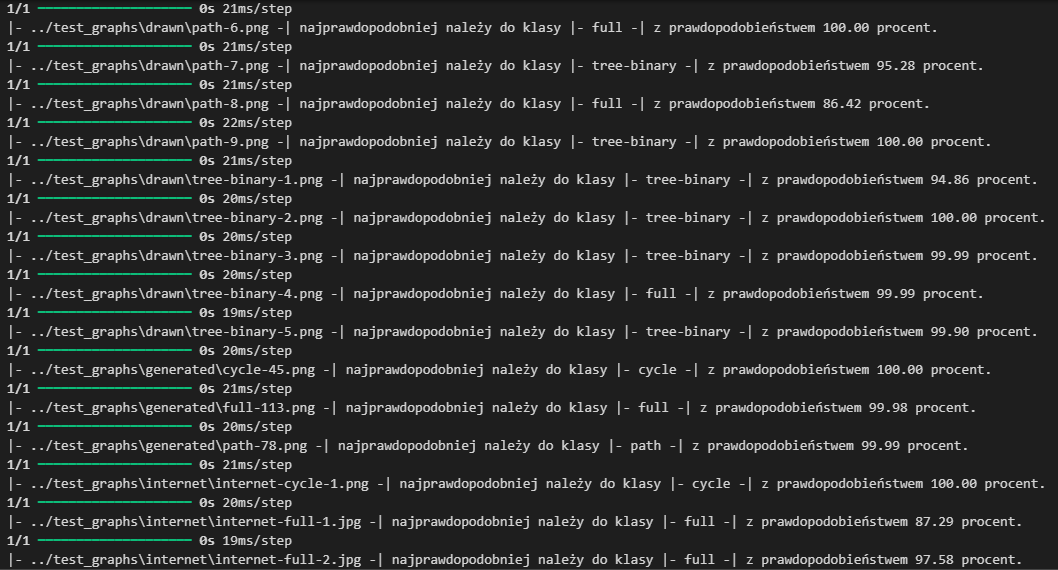
\includegraphics[width=14cm]{resources/tests/images/v4/base6_1_1_txt.png}
	\caption{Klasyfikacja obrazów zewnętrznych dla poprawionego zmodyfikowanego modelu podstawowego, liczba wierzchołków = 6}
	\label{Fig:tests-base-6b}
\end{figure}
\FloatBarrier

\begin{figure}[ht]
	\centering
	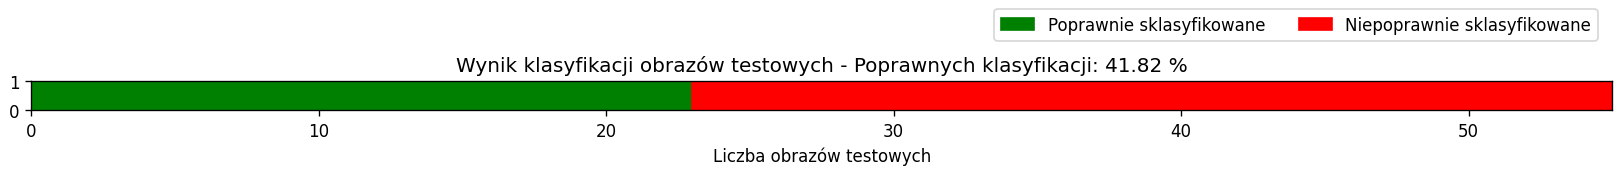
\includegraphics[width=14cm]{resources/tests/images/v4/base6_1_1_bar.png}
	\caption{Wizualizacja klasyfikacji obrazów zewnętrznych dla poprawionego zmodyfikowanego modelu podstawowego, liczba wierzchołków = 6}
	\label{Fig:tests-base-6c}
\end{figure}
\FloatBarrier

% -- TO DO -- % Opis klasyfikacji